\chapter{Background}
\label{sec:background}

As base knowledge for the algorithm, the following items must be explained. We
first describe \emph{Markov decision processes (MDPs)}, then  MCTS, then
options and finally the \emph{video game description language (VGDL)}.

\section{Markov Decision Processes}
\label{subsec:mdps}
In this paper, a game will be treated as an MDP, which is a
tuple $\langle S, A, T, R \rangle$. $S$ denotes the set of states. An MDP is
fully observable, meaning that a state contains all the information of the
game's current condition: locations of monsters, the avatar, etc. $A$ is a
finite set of actions, the input an agent can deliver to the game. $T$ is a
transition function defined as $T : S \times A \times S \rightarrow
\left[0,1\right]$. It specifies the probabilities over the possible next states,
when taking an action in a state.  $R$ is a reward function defined as $R: S
\times A \times S \rightarrow \mathbb{R}$. In this case, when the game score
increases, the increase is viewed as the reward. Algorithms typically maximize
the cumulative reward, which is analogous to the score. An MDP by definition has
the \emph{Markov property}, which means that the conditional probability
distribution of future states depends only upon the present state. No
information from previous states is needed. Algorithms do not have access to $T$
and $R$ in the scope of this paper.

\section{Monte Carlo Tree Search}
\begin{figure}
	\centering
	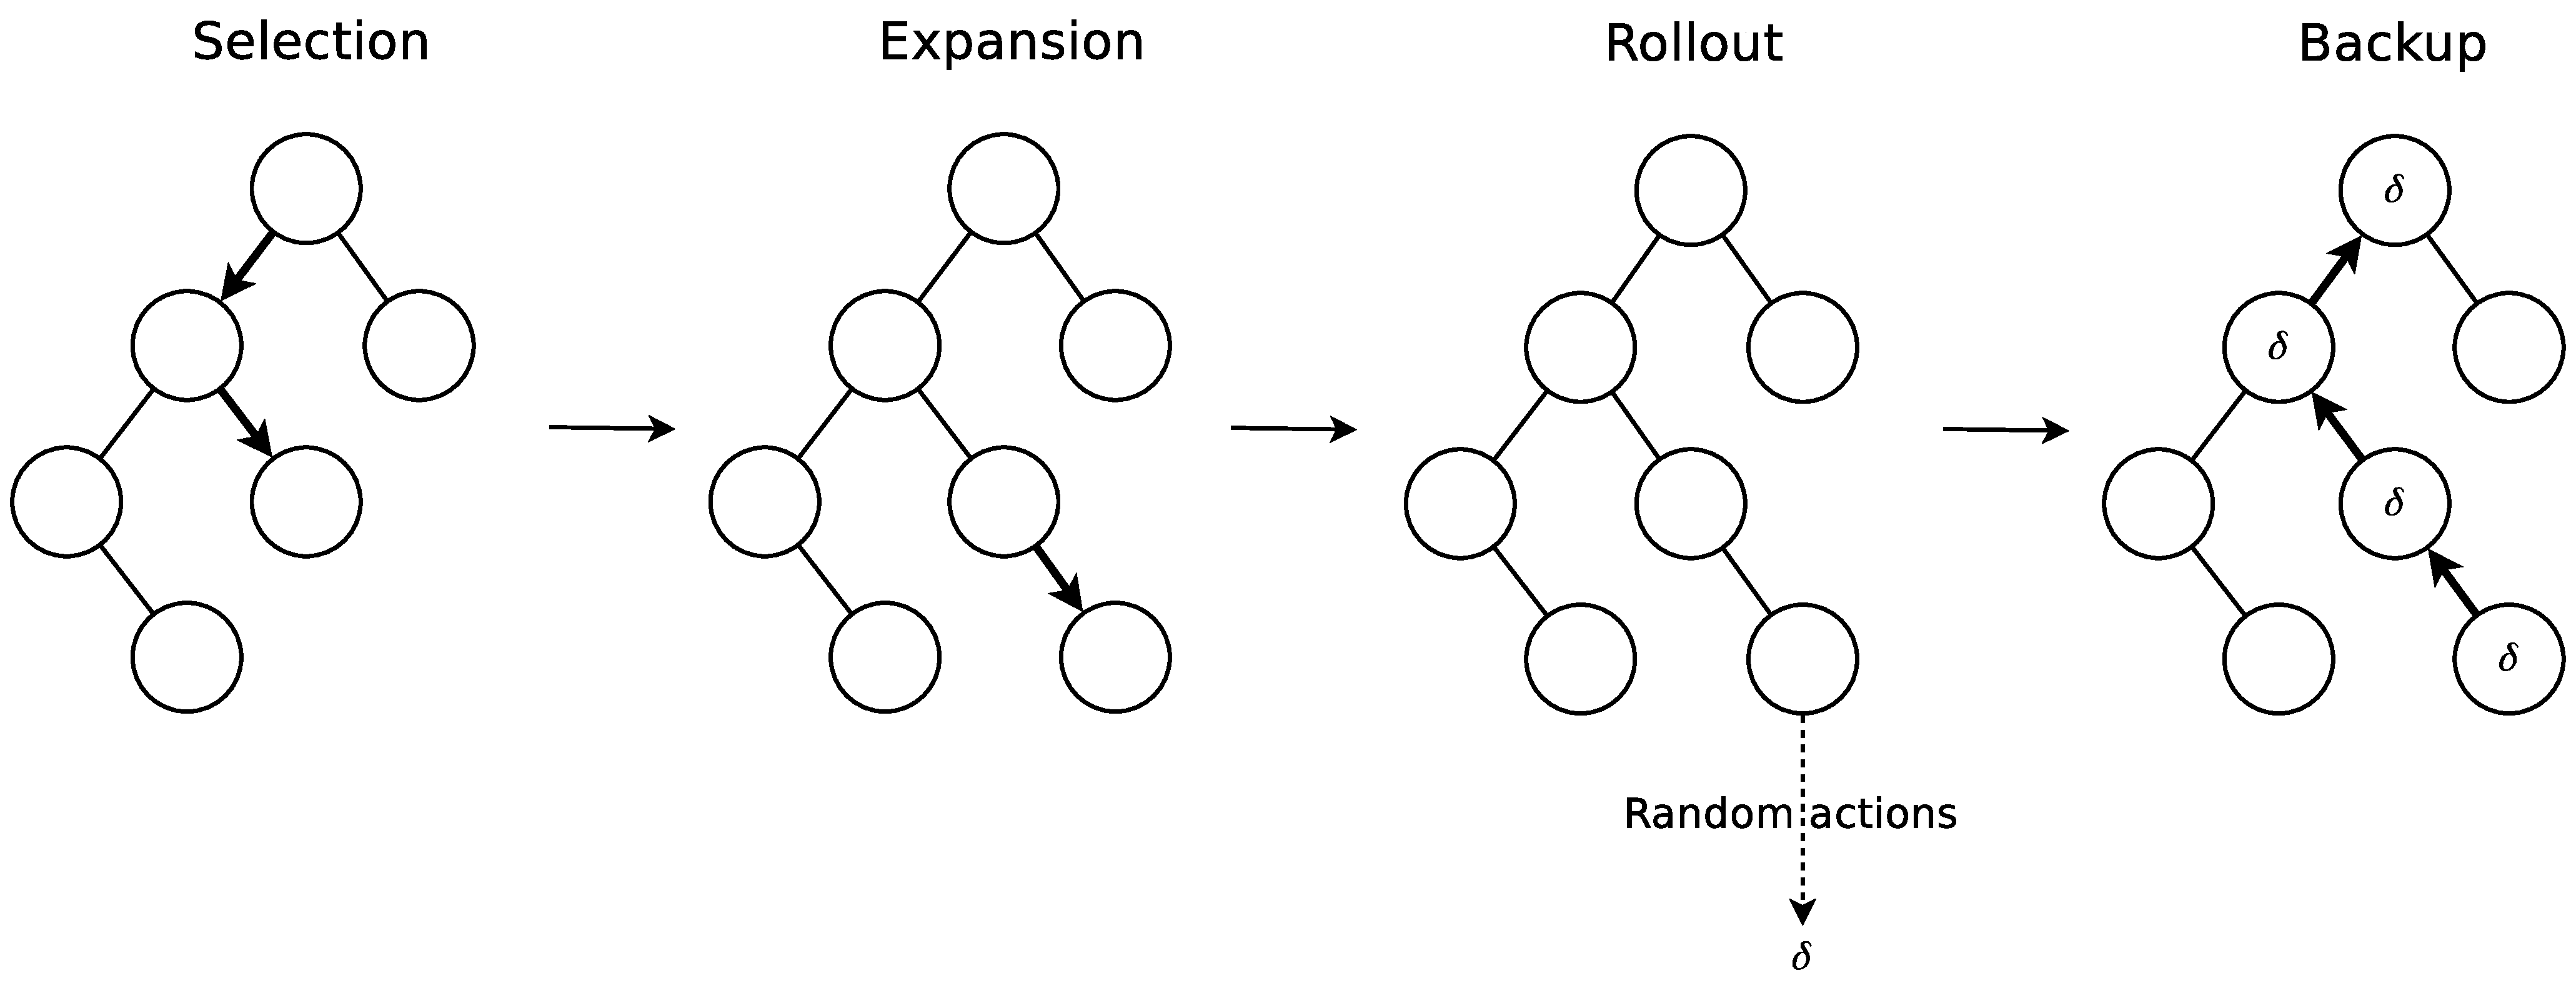
\epsfig{file=includes/mcts-wide.eps, width=\textwidth}
	\caption{One Monte Carlo tree search iteration}
	\label{fig:mcts}
\end{figure}

\label{subsec:mcts}
Monte Carlo methods have their roots in statistical physics, where they have
been used to approximate intractable integrals. Abrahamson
\cite{abramson1990expected} demonstrated theoretically that this sampling method might be
useful for action selection in games as well.  In 2001, Monte Carlo methods were
effectively used for bridge \cite{ginsberg2001gib}. The real success of MCTS
started in 2006, when the tree search method and UCT formula were introduced,
yielding very good results in Computer Go \cite{gelly2006modification}. Since
2006, the algorithm has been extended with many variations is still being used
for other computer games \cite{browne2012survey}, including the GVGAI
competition \cite{perez2014knowledge}.

This section explains how it approximates the value of actions taken in a
specific state. A tree is built incrementally from the states and actions that
are visited in a game. Each node in the tree represents a state, each connection
in the tree represents an action taken in that state leading to a state, which
is represented by the next tree node.  The process, as explained in Figure
\ref{fig:mcts}, consists of four phases that are constantly repeated. It is
started with the current game state, which is represented by the root node of
the tree. The first action is chosen by an \emph{expansion strategy} and
subsequently simulated, resulting in a new game state, for which a new node is
created. A \emph{rollout} is done from the new node, which means that a
simulation is run from the new node applying random actions until a predefined
stop criterion is met or the game ends. Finally, the score difference resulting
from the rollout is backed up, to the root node, which means that the reward is
saved to the visited nodes. Then a new iteration starts. When all actions are
expanded in a node, we call that node \emph{fully expanded} and use a
\emph{selection strategy} to select a next node. When a node is selected that is
not fully expanded, the expansion strategy is used to create a new node, after
which a rollout takes place and the results are backed up thereafter.

	%(Term from pMCTS.pdf)
The selection strategy selects optimal actions in internal tree nodes, depending
on the values of the child nodes. An effective and very popular selection
strategy is the \emph{upper confidence tree (UCT)} \cite{kocsis2006bandit},
which balances the choice between poorly explored actions with a high
uncertainty about their value and actions that have been explored but have a
higher value. A child node $j$ is selected to maximize
\begin{equation}
	\label{eq:uct}
	UCT = 2C_p \sqrt{\frac{2 \ln n_s}{n_{s'}}}
\end{equation}
Where $n_s$ is the number of times the current node $s$ has been visited,
$n_{s'}$ is the number of times child $c$ has been visited and $C_p > 0$ is a
constant, often set to $\sqrt{2}$, that shifts priority from exploration to
exploitation.

The traditional expansion strategy is to explore each action at least once in
each node. After all actions have been expanded, the node applies the selection
strategy for further exploration. Some variants of MCTS reduce the branching
factor of the tree by only expanding the nodes selected by a special expansion
strategy. A specific example is the \emph{crazy stone} algorithm
\cite{coulom2007efficient}, which is an expansion strategy that was designed
specifically for Go. We will use an adaptation of this strategy in the algorithm
proposed in Section \ref{sec:learning}.  When using crazy stone, an action $i$
is selected with a probability proportional to $u_i$
\begin{equation}
	\label{eq:crazystone}
	u_i = \exp\left(K \frac{\mu_0 - \mu_i}{\sqrt{2\left(\sigma_0^2 +
\sigma_i^2\right)}}\right) + \epsilon_i
\end{equation}
Each action has an estimated value $\mu_i$ ordered in such a way that $\mu_0 >
\mu_1 > \ldots > \mu_N$, and a variance $\sigma_i^2$. $\epsilon_i$ prevents 
the probability of selecting a move to reach zero and its value is proportional to
the ordering of the expected values of the possible actions. K is a constant
that influences the exploration/exploitation trade off.
\begin{equation}
	\label{eq:epsilon}
	\epsilon_i = \frac{0.1 + 2^{-i} + a_i}{N}
\end{equation}
Where $a_i$ is 1 when an action is \emph{an atari move}, a go-specific
move that can otherwise easily be underestimated by MCTS, and otherwise 0.

After a rollout, the reward is backed up, which means that the estimated value
for every node that has been visited in this iteration is updated with the
reward of this simulation. Usually the estimated value of a node is the average
of all rewards backed up to that node.

\section{Options}
\label{subsec:options}
%\todo{Options}
For mimicking human game playing strategies like defining and solving subgoals
and subtasks, we use options \cite{sutton1999between, barto2003recent}. An
option is a predefined method of reaching a specific subgoal. Formally, it is a
triple $\langle I, \pi, \beta\rangle$ in which $I \subseteq S$ is an initiation
set, $\pi: S \times A \rightarrow [0, 1]$ is a policy and $\beta: S^+
\rightarrow[0,1]$ is a termination condition.

A policy $\pi$ defines the action that should be taken in a state. The
initiation set $I$ is a set of states in which the option can be started. When the
option starts, policy $\pi$ will be followed, until a state is reached that
satisfies a termination condition in $\beta$. Using options in an MDP removes
the Markov property for that process: the state information alone is no longer
enough to predict an agent's actions, since the actions are now not only
state-dependant, but dependant on what option the agent has chosen in the past
as well. The process is now called a \emph{semi-Markov decision process
(SMDP)}. For convenience, we will call the original action set of the MDP $A$,
and the set of options $O$.  Normal actions can be treated as options as well.
An option for action $a \in A$ has a initiation set $I = S$, the policy $\pi$ is
taking action $a$ in all the states. The termination condition $\beta$ is that
action $a$ should be performed once.

\section{Video Game Description Language}
\label{subsec:vgdl}
This paper will use a framework called the video game description
language \cite{schaul2013video}, in which games can very easily be defined.

To define a game in VGDL, two files should be created. Firstly, the game
description should be made, which defines for each type of object what its
character in the level description is, what it looks like in the game, how it
interacts with other objects and the world, and when it disappears from the
game. Secondly, a level description should be made, in which each character maps
to an object in the game, on the same grid location as the character has in the
file. By only defining these two files a wide spectrum of games can be created.

In this paper, we will use a Java implementation made for the GVGAI competition,
which comes with many games. The algorithm proposed in this paper will be
benchmarked on these games, using the rules of the GVGAI competition. 
